\documentclass[10pt,aspectratio=169]{beamer}

% -----------------------------------------------------------------------------
% Visual system: Graphite--Teal--Saffron
% Compile from the directory containing this file:
%   pdflatex visual-sketchpad-9.5.tex
% Run twice so the total frame count is resolved.
% -----------------------------------------------------------------------------
\usetheme{default}
\usefonttheme{professionalfonts}

\usepackage[T1]{fontenc}
\usepackage[utf8]{inputenc}
\IfFileExists{sourcesanspro.sty}
  {\usepackage[sfdefault]{sourcesanspro}}
  {\usepackage{lmodern}}
\IfFileExists{sourcecodepro.sty}{\usepackage[scaled=0.88]{sourcecodepro}}{}

\usepackage{amsmath,amssymb}
\usepackage{booktabs}
\usepackage{array}
\usepackage{colortbl}
\usepackage{graphicx}
\usepackage{listings}
\usepackage{tabularx}
\usepackage{tikz}
\usetikzlibrary{arrows.meta,positioning,calc,fit,backgrounds}
\IfFileExists{microtype.sty}{\usepackage{microtype}}{}

\graphicspath{{visual-sketchpad-figures/}{figures/}}

% --- Palette -----------------------------------------------------------------
\definecolor{Ink}{HTML}{1D2733}
\definecolor{Teal}{HTML}{0B6B69}
\definecolor{TealDark}{HTML}{075250}
\definecolor{Saffron}{HTML}{D8A12E}
\definecolor{Paper}{HTML}{F7F8FA}
\definecolor{Mist}{HTML}{EDF1F3}
\definecolor{MistDeep}{HTML}{D9E1E5}
\definecolor{Muted}{HTML}{65717C}
\definecolor{Forest}{HTML}{2F7D5C}
\definecolor{Rust}{HTML}{B44A3A}

\setbeamercolor{background canvas}{bg=Paper}
\setbeamercolor{normal text}{fg=Ink,bg=Paper}
\setbeamercolor{structure}{fg=Teal}
\setbeamercolor{frametitle}{fg=Ink,bg=Paper}
\setbeamercolor{alerted text}{fg=Rust}
\setbeamercolor{block title}{fg=white,bg=Teal}
\setbeamercolor{block body}{fg=Ink,bg=white}
\setbeamercolor{footline}{fg=Muted,bg=Paper}
\setbeamercolor{progress line}{bg=Teal}
\setbeamercolor{card}{fg=Ink,bg=white}
\setbeamercolor{soft card}{fg=Ink,bg=Mist}
\setbeamercolor{accent card}{fg=Ink,bg=Saffron!18}
\setbeamercolor{positive card}{fg=Ink,bg=Teal!9}
\setbeamercolor{negative card}{fg=Ink,bg=Rust!8}

\setbeamerfont{normal text}{size=\fontsize{10.8}{13.2}\selectfont}
\setbeamerfont{frametitle}{series=\bfseries,size=\fontsize{17}{19}\selectfont}
\setbeamerfont{section in head/foot}{series=\bfseries,size=\fontsize{7.5}{9}\selectfont}
\setbeamerfont{footline}{size=\fontsize{7.5}{9}\selectfont}
\setbeamerfont{caption}{size=\scriptsize}

\setbeamertemplate{navigation symbols}{}
\setbeamertemplate{blocks}[rounded][shadow=false]
\setbeamertemplate{itemize item}{\raise0.15ex\hbox{\color{Teal}\scriptsize$\blacktriangleright$}}
\setbeamertemplate{itemize subitem}{\raise0.1ex\hbox{\color{Saffron}\tiny$\bullet$}}
\setbeamertemplate{enumerate item}{\color{Teal}\bfseries\insertenumlabel.}
\setbeamersize{text margin left=0.65cm,text margin right=0.65cm}

% --- Frame title and footer ---------------------------------------------------
\setbeamertemplate{frametitle}{%
  \nointerlineskip
  \begin{beamercolorbox}[wd=\paperwidth,leftskip=0.65cm,rightskip=0.65cm,sep=0pt]{frametitle}
    \par\vskip0.30cm\nointerlineskip
    {\usebeamerfont{section in head/foot}\color{Teal}\MakeUppercase{\insertsectionhead}\par}
    \vspace{0.00cm}
    {\usebeamerfont{frametitle}\insertframetitle\par}
    \vspace{0.02cm}
    {\color{Saffron}\rule{1.05cm}{1.25pt}}
    \vspace{-0.26cm}
  \end{beamercolorbox}%
}

\setbeamertemplate{footline}{%
  \leavevmode
  \begin{beamercolorbox}[wd=\paperwidth,ht=0.7pt,dp=0pt]{progress line}\end{beamercolorbox}
  \begin{beamercolorbox}[wd=\paperwidth,ht=2.6ex,dp=1.15ex,leftskip=0.65cm,rightskip=0.65cm]{footline}
    \usebeamerfont{footline}\insertshorttitle
    \hfill
    \insertsectionhead\hspace{0.8em}\textcolor{MistDeep}{|}\hspace{0.8em}
    \insertframenumber/\inserttotalframenumber
  \end{beamercolorbox}%
}

% --- Reusable components ------------------------------------------------------
\newcommand{\name}{\textsc{Sketchpad}}
\newcommand{\eyebrow}[1]{%
  {\color{Teal}\bfseries\fontsize{8}{9.5}\selectfont\MakeUppercase{#1}}%
}
\newcommand{\source}[1]{%
  \begin{tikzpicture}[remember picture,overlay]
    \node[anchor=south east,text=Muted,
          font=\fontsize{6.4}{7.4}\selectfont]
      at ($(current page.south east)+(-0.67cm,0.54cm)$)
      {\parbox{12.0cm}{\raggedleft #1\par}};
  \end{tikzpicture}%
}
\newcommand{\pill}[1]{%
  \tikz[baseline=(P.base)]\node[rounded corners=2pt,fill=Teal!10,
    inner xsep=6pt,inner ysep=2.5pt,text=TealDark,font=\scriptsize\bfseries] (P) {#1};%
}
\newcommand{\goldpill}[1]{%
  \tikz[baseline=(P.base)]\node[rounded corners=2pt,fill=Saffron!22,
    inner xsep=6pt,inner ysep=2.5pt,text=Ink,font=\scriptsize\bfseries] (P) {#1};%
}
\newcommand{\upcell}[1]{\cellcolor{Teal!10}\textcolor{TealDark}{\bfseries +#1}}
\newcommand{\downcell}[1]{\cellcolor{Rust!8}\textcolor{Rust}{\bfseries #1}}

\lstset{
  language=Python,
  basicstyle=\ttfamily\fontsize{8.3}{10.2}\selectfont,
  keywordstyle=\color{TealDark}\bfseries,
  commentstyle=\color{Muted}\itshape,
  stringstyle=\color{Rust},
  showstringspaces=false,
  breaklines=true,
  frame=none,
  backgroundcolor=\color{Mist},
  xleftmargin=0.35cm,
  xrightmargin=0.25cm,
  aboveskip=0.15cm,
  belowskip=0.15cm
}

% A compact paired-dot result row. Use inside a TikZ picture with x/y scales.
\newcommand{\resultrow}[4]{%
  \node[anchor=east,xshift=-0.20cm,
        font=\scriptsize\bfseries,text=Ink] at (0,#4) {#1};
  \draw[MistDeep,line width=1.8pt] (0,#4) -- (100,#4);
  \draw[Saffron,line width=2.2pt] (#2,#4) -- (#3,#4);
  \fill[Muted] (#2,#4) circle (2.35pt);
  \fill[Teal] (#3,#4) circle (3.05pt);
  \node[anchor=north east,yshift=-1.2pt,font=\fontsize{6.7}{7.5}\selectfont,
        text=Muted] at (#2,#4) {#2};
  \node[anchor=south west,yshift=1.2pt,font=\fontsize{6.7}{7.5}\selectfont\bfseries,
        text=TealDark] at (#3,#4) {#3};
}

% --- Metadata ----------------------------------------------------------------
\title[IPL Lab]{Visual Sketchpad}
\subtitle{Sketching as a Visual Chain of Thought for Multimodal Language Models}
\author[Shayan Salehi]{Shayan Salehi}
\institute[SUT]{Department of Computer Engineering\\Sharif University of Technology}
\date{July 2026}

\begin{document}

% =============================================================================
% 01 — TITLE
% =============================================================================
{
\setbeamercolor{background canvas}{bg=Ink}
\begin{frame}[plain]
  \begin{tikzpicture}[remember picture,overlay]
    \fill[Teal!34!Ink]
      ($(current page.north east)+(-5.35cm,0)$) rectangle (current page.south east);
    \fill[Saffron]
      ($(current page.north west)+(0,-0.42cm)$) rectangle
      ($(current page.north west)+(1.35cm,-0.49cm)$);
    \draw[white!7,line width=0.7pt,step=0.55cm]
      ($(current page.north east)+(-5.35cm,0)$) grid (current page.south east);
  \end{tikzpicture}

  \vspace{0.66cm}
  \begin{columns}[T,onlytextwidth]
    \column{0.57\textwidth}
      {\color{Saffron}\bfseries\fontsize{8.5}{10}\selectfont
       IPL LAB PRESENTATION}\par
      \vspace{0.52cm}
      {\color{white}\bfseries\fontsize{29}{31}\selectfont Visual Sketchpad}\par
      \vspace{0.20cm}
      {\color{white!78}\fontsize{14}{17}\selectfont
       Sketching as a Visual Chain of Thought\\
       for Multimodal Language Models}\par
      \vspace{0.72cm}
      {\color{white}\bfseries Shayan Salehi}\par
      {\color{white!63}\small Department of Computer Engineering\\
       Sharif University of Technology}\par
      \vspace{0.46cm}
      {\color{white!45}\scriptsize June 2026 \quad\textbullet\quad
       Hu et al., NeurIPS 2024}

    \column{0.43\textwidth}
      \centering
      \vspace{0.34cm}
      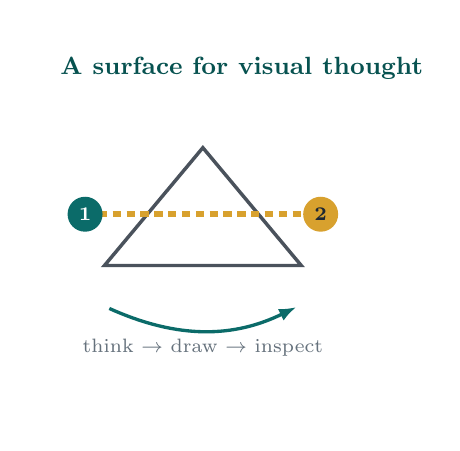
\begin{tikzpicture}[scale=0.88,>=Latex]
        \node[rounded corners=7pt,fill=white,minimum width=4.45cm,
              minimum height=5.02cm] (pad) at (0,0) {};
        \node[anchor=north west,text=TealDark,font=\bfseries\small]
              at ($(pad.north west)+(0.34,-0.30)$) {A surface for visual thought};
        \draw[Ink!80,line width=1.25pt]
              (-1.42,-0.58) -- (0,1.12) -- (1.42,-0.58) -- cycle;
        \draw[Saffron,line width=2pt,densely dashed]
              (-1.70,0.16) -- (1.70,0.16);
        \node[circle,fill=Teal,text=white,font=\scriptsize\bfseries,
              inner sep=2.2pt] at (-1.70,0.16) {1};
        \node[circle,fill=Saffron,text=Ink,font=\scriptsize\bfseries,
              inner sep=2.2pt] at (1.70,0.16) {2};
        \draw[Teal,line width=1.2pt,-{Latex[length=2.2mm]}]
              (-1.35,-1.20) .. controls (-0.35,-1.65) and (0.45,-1.62) .. (1.35,-1.18);
        \node[text=Muted,font=\scriptsize,align=center]
              at (0,-1.76) {think $\rightarrow$ draw $\rightarrow$ inspect};
      \end{tikzpicture}
  \end{columns}
\end{frame}
}

% =============================================================================
\section{Premise}
% =============================================================================

% 02 — THESIS / ROADMAP
\begin{frame}{Give the model a surface to draw on}
  \vspace{0.25cm}
  \begin{center}
    {\fontsize{21}{25}\selectfont\bfseries
     A visual artifact can be both a \textcolor{Teal}{reasoning step}
     and a \textcolor{Saffron!90!black}{new observation}.}
  \end{center}
  \vspace{0.58cm}

  \begin{columns}[T,onlytextwidth]
    \column{0.315\textwidth}
      \begin{beamercolorbox}[rounded=true,wd=\linewidth,ht=2.35cm,dp=0.20cm,sep=0.27cm]{card}
        \eyebrow{01 \; Premise}\par\vspace{0.18cm}
        {\bfseries Humans externalize spatial structure by drawing.}\par
        \vspace{0.12cm}{\small Why should multimodal LMs reason only in text?}
      \end{beamercolorbox}
    \column{0.315\textwidth}
      \begin{beamercolorbox}[rounded=true,wd=\linewidth,ht=2.35cm,dp=0.20cm,sep=0.27cm]{positive card}
        \eyebrow{02 \; Mechanism}\par\vspace{0.18cm}
        {\bfseries Thought, action, and observation remain multimodal.}\par
        \vspace{0.12cm}{\small The model plans, draws, inspects, and adapts.}
      \end{beamercolorbox}
    \column{0.315\textwidth}
      \begin{beamercolorbox}[rounded=true,wd=\linewidth,ht=2.35cm,dp=0.20cm,sep=0.27cm]{accent card}
        \eyebrow{03 \; Evidence}\par\vspace{0.18cm}
        {\bfseries The gain is largest when the missing representation is visual.}\par
        \vspace{0.12cm}{\small Math, search, depth, and correspondence all improve.}
      \end{beamercolorbox}
  \end{columns}
\end{frame}

% 03 — MOTIVATION
\begin{frame}{Sketches externalize structure that language must reconstruct}
  \begin{columns}[T,onlytextwidth]
    \column{0.55\textwidth}
      \centering
      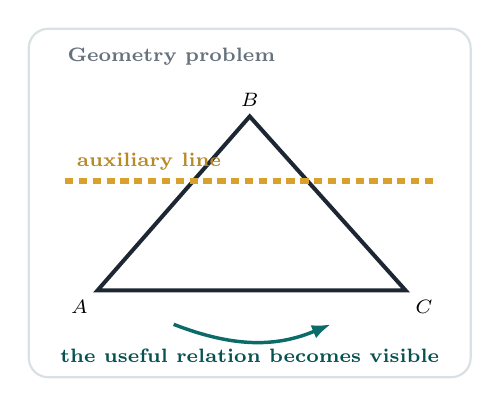
\begin{tikzpicture}[scale=0.92]
        \fill[white,rounded corners=7pt] (-3.05,-2.45) rectangle (3.05,2.36);
        \draw[MistDeep,line width=0.8pt,rounded corners=7pt] (-3.05,-2.45) rectangle (3.05,2.36);
        \node[anchor=west,font=\scriptsize\bfseries,text=Muted] at (-2.65,1.98)
              {Geometry problem};
        \draw[Ink,line width=1.45pt] (-2.10,-1.25) -- (0,1.15) -- (2.15,-1.25) -- cycle;
        \node[above,font=\scriptsize\bfseries] at (0,1.15) {$B$};
        \node[below left,font=\scriptsize\bfseries] at (-2.10,-1.25) {$A$};
        \node[below right,font=\scriptsize\bfseries] at (2.15,-1.25) {$C$};
        \draw[Saffron,line width=2.4pt,densely dashed] (-2.55,0.26) -- (2.55,0.26);
        \node[anchor=west,text=Saffron!85!black,font=\scriptsize\bfseries]
              at (-2.52,0.52) {auxiliary line};
        \draw[Teal,line width=1.25pt,-{Latex[length=2.4mm]}]
              (-1.05,-1.72) .. controls (-0.20,-2.05) and (0.38,-2.03) .. (1.12,-1.72);
        \node[text=TealDark,font=\scriptsize\bfseries] at (0,-2.16)
              {the useful relation becomes visible};
      \end{tikzpicture}

    \column{0.42\textwidth}
      \vspace{0.15cm}
      {\fontsize{16}{19}\selectfont\bfseries
       Drawing is cognitive scaffolding.}\par
      \vspace{0.24cm}
      \begin{itemize}
        \setlength{\itemsep}{0.25cm}
        \item \textbf{Geometry:} add support lines and expose angle relations.
        \item \textbf{Search:} crop, circle, and inspect small regions.
        \item \textbf{Perception:} turn depth, masks, and correspondence into visible evidence.
      \end{itemize}
  \end{columns}
\end{frame}

% 04 — GAP
\begin{frame}{Text-only intermediates discard the structure}
  \vspace{0.20cm}
  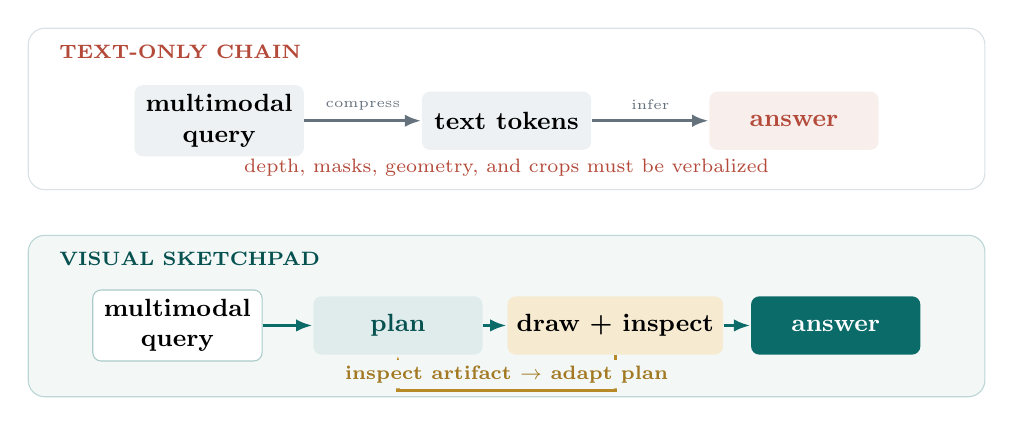
\begin{tikzpicture}[>=Latex,node distance=0.48cm and 0.62cm]
    \tikzset{
      lane/.style={rounded corners=6pt,minimum width=12.15cm,minimum height=2.05cm,draw=MistDeep,fill=white},
      pipebox/.style={rounded corners=3pt,minimum width=2.15cm,minimum height=0.74cm,
                   align=center,font=\small\bfseries},
      arr/.style={-{Latex[length=2.1mm]},line width=1.2pt}
    }
    \node[lane] (old) at (0,1.35) {};
    \node[anchor=west,font=\scriptsize\bfseries,text=Rust] at ($(old.west)+(0.28,0.72)$)
          {TEXT-ONLY CHAIN};
    \node[pipebox,fill=Mist] (q1) at (-3.65,1.20) {multimodal\\query};
    \node[pipebox,fill=Mist] (t1) at (0,1.20) {text tokens};
    \node[pipebox,fill=Rust!9,text=Rust] (a1) at (3.65,1.20) {answer};
    \draw[arr,draw=Muted] (q1) -- node[above,font=\tiny,text=Muted] {compress} (t1);
    \draw[arr,draw=Muted] (t1) -- node[above,font=\tiny,text=Muted] {infer} (a1);
    \node[font=\scriptsize,text=Rust] at (0,0.60)
          {depth, masks, geometry, and crops must be verbalized};

    \node[lane,fill=Teal!5,draw=Teal!28] (new) at (0,-1.28) {};
    \node[anchor=west,font=\scriptsize\bfseries,text=TealDark] at ($(new.west)+(0.28,0.72)$)
          {VISUAL SKETCHPAD};
    \node[pipebox,fill=white,draw=Teal!35] (q2) at (-4.18,-1.40) {multimodal\\query};
    \node[pipebox,fill=Teal!13,text=TealDark] (p2) at (-1.38,-1.40) {plan};
    \node[pipebox,fill=Saffron!22] (s2) at (1.38,-1.40) {draw + inspect};
    \node[pipebox,fill=Teal,text=white] (a2) at (4.18,-1.40) {answer};
    \draw[arr,draw=Teal] (q2) -- (p2);
    \draw[arr,draw=Teal] (p2) -- (s2);
    \draw[arr,draw=Teal] (s2) -- (a2);
    \draw[arr,draw=Saffron!85!black] (s2.south) -- ++(0,-0.45) -| (p2.south);
    \node[rounded corners=2pt,fill=Teal!5,inner xsep=4pt,inner ysep=2pt,
          font=\scriptsize\bfseries,text=Saffron!75!black]
          at (0,-2.02) {inspect artifact $\rightarrow$ adapt plan};
  \end{tikzpicture}
\end{frame}

% 05 — CONTRIBUTIONS
\begin{frame}{Visual Sketchpad adds an adaptive reasoning}
  \vspace{0.16cm}
  \begin{columns}[T,onlytextwidth]
    \column{0.315\textwidth}
      \begin{beamercolorbox}[rounded=true,wd=\linewidth,ht=3.35cm,dp=0.18cm,sep=0.28cm]{positive card}
        {\fontsize{23}{25}\selectfont\bfseries\textcolor{Teal}{01}}\par
        \vspace{0.14cm}{\bfseries Mixed visual chain of thought}\par
        \vspace{0.17cm}{\small Plans, programs, images, and text coexist in the same iterative context.}
      \end{beamercolorbox}
    \column{0.315\textwidth}
      \begin{beamercolorbox}[rounded=true,wd=\linewidth,ht=3.35cm,dp=0.18cm,sep=0.28cm]{card}
        {\fontsize{23}{25}\selectfont\bfseries\textcolor{Teal}{02}}\par
        \vspace{0.14cm}{\bfseries Specialist vision tools}\par
        \vspace{0.17cm}{\small Detection, segmentation, depth, search, crop, and overlay become sketching primitives.}
      \end{beamercolorbox}
    \column{0.315\textwidth}
      \begin{beamercolorbox}[rounded=true,wd=\linewidth,ht=3.35cm,dp=0.18cm,sep=0.28cm]{accent card}
        {\fontsize{23}{25}\selectfont\bfseries\textcolor{Saffron!85!black}{03}}\par
        \vspace{0.14cm}{\bfseries Training-free evidence}\par
        \vspace{0.17cm}{\small Reported average gains of \textbf{12.7\%} on math and \textbf{8.6\%} on vision tasks.}
      \end{beamercolorbox}
  \end{columns}
  \vspace{0.28cm}
  \begin{center}
    \pill{no finetuning}\hspace{0.25cm}
    \pill{implemented with AutoGen}\hspace{0.25cm}
    \goldpill{state of the art on all tested vision tasks}
  \end{center}
\end{frame}

% 06 — HERO FIGURE
\begin{frame}{When the model draws the missing representation}
  \vspace{0.03cm}
  \begin{columns}[T,onlytextwidth]
    \column{0.49\textwidth}
      \centering
      \includegraphics[width=\linewidth,trim=0 880 1200 0,clip]{teaser-small.pdf}
    \column{0.49\textwidth}
      \centering
      \includegraphics[width=\linewidth,trim=1200 0 0 833,clip]{teaser-small.pdf}
  \end{columns}
\end{frame}

% =============================================================================
\section{Mechanism}
% =============================================================================

% 07 — LOOP
\begin{frame}{Sketchpad turns reasoning into a feedback loop}
  \centering
  \vspace{0.14cm}
  \resizebox{0.93\textwidth}{!}{%
  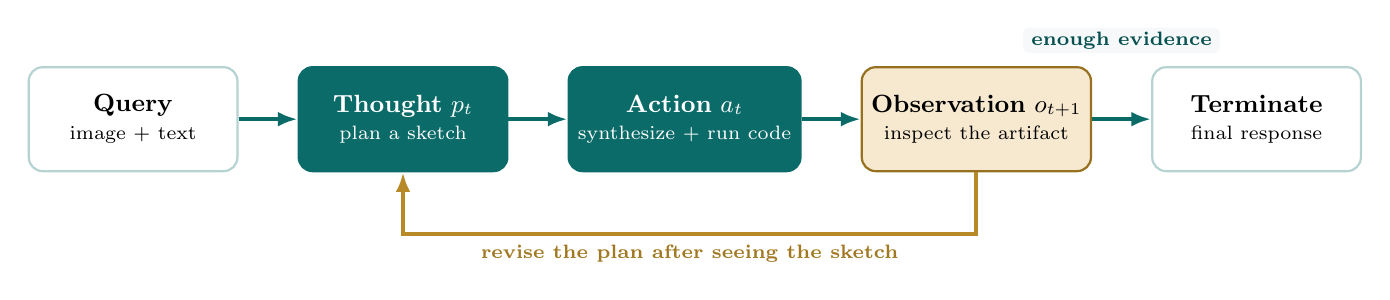
\begin{tikzpicture}[>=Latex,node distance=0.75cm]
    \tikzset{
      stage/.style={rounded corners=5pt,minimum width=2.65cm,minimum height=1.32cm,
                    align=center,font=\small,draw=Teal!30,line width=0.8pt,fill=white},
      active/.style={stage,fill=Teal,text=white,draw=Teal},
      artifact/.style={stage,fill=Saffron!23,draw=Saffron!70!black},
      flow/.style={-{Latex[length=2.5mm]},line width=1.4pt,draw=Teal}
    }
    \node[stage] (query) {\textbf{Query}\\[-1pt]\scriptsize image + text};
    \node[active,right=of query] (thought) {\textbf{Thought} $p_t$\\[-1pt]\scriptsize plan a sketch};
    \node[active,right=of thought] (action) {\textbf{Action} $a_t$\\[-1pt]\scriptsize synthesize + run code};
    \node[artifact,right=of action] (obs) {\textbf{Observation} $o_{t+1}$\\[-1pt]\scriptsize inspect the artifact};
    \node[stage,right=of obs] (answer) {\textbf{Terminate}\\[-1pt]\scriptsize final response};
    \draw[flow] (query) -- (thought);
    \draw[flow] (thought) -- (action);
    \draw[flow] (action) -- (obs);
    \draw[flow] (obs) -- (answer);
    \node[rounded corners=2pt,fill=Paper,inner xsep=3pt,inner ysep=1.5pt,
          font=\scriptsize\bfseries,text=TealDark]
          at ($(obs.east)!0.5!(answer.west)+(0,1.00)$) {enough evidence};
    \draw[-{Latex[length=2.5mm]},line width=1.5pt,draw=Saffron!85!black]
      (obs.south) -- ++(0,-0.78) -| node[below,pos=0.25,font=\scriptsize\bfseries,
      text=Saffron!75!black] {revise the plan after seeing the sketch} (thought.south);
  \end{tikzpicture}}
  \vspace{0.42cm}
  \begin{columns}[onlytextwidth]
    \column{0.31\textwidth}\centering\pill{multimodal observations}
    \column{0.31\textwidth}\centering\pill{executable actions}
    \column{0.31\textwidth}\centering\goldpill{error-aware replanning}
  \end{columns}
\end{frame}

% 08 — FRAMEWORK FIGURE
\begin{frame}{Supports geometry, graphs, search, and depth tools}
  \centering
  \vspace{0.02cm}
  \includegraphics[height=0.59\textheight]{framework.pdf}
\end{frame}

% 09 — CODE GENERATION
\begin{frame}[fragile]{Tool signatures become executable sketches}
  \begin{columns}[T,onlytextwidth]
    \column{0.48\textwidth}
      \eyebrow{What the model receives}\par
      \vspace{0.10cm}
      {\small Function signatures and docstrings---not specialist implementations.}
      \vspace{0.10cm}
\begin{lstlisting}
# Generated during inference
depth_map = depth(image)
overlay = overlay_images(
    depth_map, image, alpha=0.55
)
display(overlay)
\end{lstlisting}
      \vspace{0.08cm}
      \begin{beamercolorbox}[rounded=true,wd=\linewidth,sep=0.18cm]{positive card}
        \textbf{Key interface:} \texttt{display()} places the new image back into the next observation.
      \end{beamercolorbox}

    \column{0.48\textwidth}
      \eyebrow{What the model gets back}\par
      \vspace{0.08cm}
      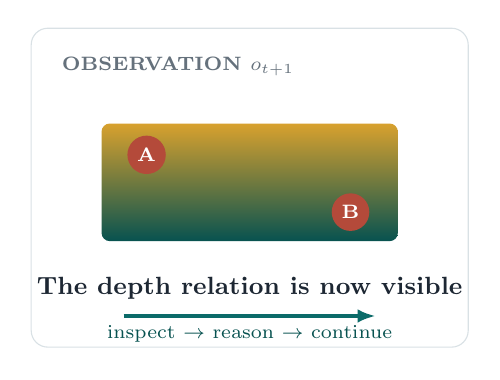
\begin{tikzpicture}[>=Latex,scale=0.97]
        \node[rounded corners=6pt,fill=white,draw=MistDeep,minimum width=5.55cm,
              minimum height=4.05cm] (canvas) at (0,0) {};
        \node[anchor=north west,font=\scriptsize\bfseries,text=Muted]
              at ($(canvas.north west)+(0.28,-0.26)$) {OBSERVATION $o_{t+1}$};
        \shade[top color=Saffron,bottom color=TealDark,rounded corners=3pt]
              (-1.94,-0.70) rectangle (1.94,0.84);
        \foreach \x/\y/\t in {-1.35/0.43/A,1.32/-0.32/B}{
          \node[circle,fill=Rust,text=white,font=\scriptsize\bfseries,inner sep=2pt]
                at (\x,\y) {\t};
        }
        \node[align=center,font=\small\bfseries,text=Ink] at (0,-1.32)
              {The depth relation is now visible};
        \draw[Teal,line width=1.4pt,-{Latex[length=2.3mm]}]
              (-1.65,-1.68) -- (1.65,-1.68);
        \node[below,font=\scriptsize,text=TealDark] at (0,-1.68)
              {inspect $\rightarrow$ reason $\rightarrow$ continue};
      \end{tikzpicture}
  \end{columns}
\end{frame}

% 10 — TOOL GALLERY
\begin{frame}{Models become a compact vocabulary of visual actions}
  \centering
  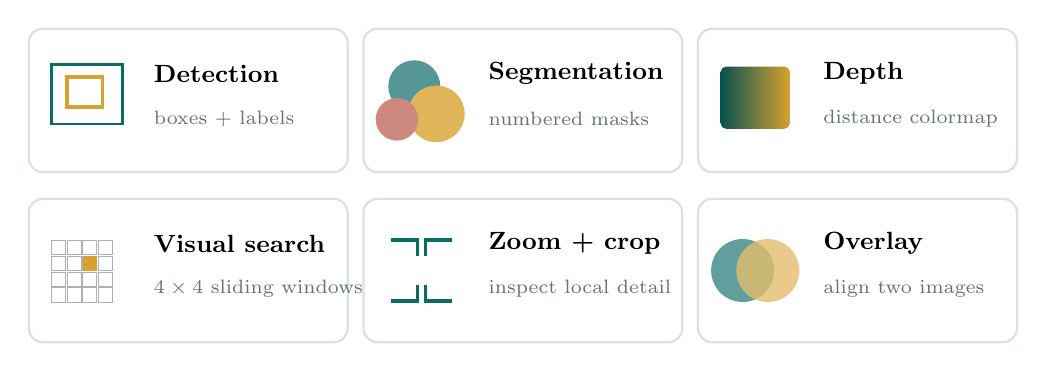
\begin{tikzpicture}
    \tikzset{tool/.style={rounded corners=5pt,fill=white,draw=MistDeep,
      line width=0.8pt,minimum width=4.05cm,minimum height=1.82cm}}
    \foreach \x/\y/\id in {-4.25/1.08/det,0/1.08/seg,4.25/1.08/dep,
                             -4.25/-1.08/search,0/-1.08/crop,4.25/-1.08/over}{
      \node[tool] (\id) at (\x,\y) {};
    }

    % Detection
    \draw[Teal,line width=1pt] ($(det.west)+(0.30,-0.30)$) rectangle ($(det.west)+(1.20,0.46)$);
    \draw[Saffron,line width=1.4pt] ($(det.west)+(0.50,-0.08)$) rectangle ($(det.west)+(0.95,0.30)$);
    \node[anchor=west,font=\small\bfseries] at ($(det.west)+(1.48,0.34)$) {Detection};
    \node[anchor=west,font=\scriptsize,text=Muted] at ($(det.west)+(1.48,-0.23)$) {boxes + labels};

    % Segmentation
    \fill[Teal!70] ($(seg.west)+(0.66,0.18)$) circle (0.33cm);
    \fill[Saffron!80] ($(seg.west)+(0.94,-0.17)$) circle (0.36cm);
    \fill[Rust!65] ($(seg.west)+(0.44,-0.24)$) circle (0.27cm);
    \node[anchor=west,font=\small\bfseries] at ($(seg.west)+(1.48,0.34)$) {Segmentation};
    \node[anchor=west,font=\scriptsize,text=Muted] at ($(seg.west)+(1.48,-0.23)$) {numbered masks};

    % Depth
    \shade[left color=TealDark,right color=Saffron,rounded corners=2pt]
      ($(dep.west)+(0.30,-0.36)$) rectangle ($(dep.west)+(1.18,0.43)$);
    \node[anchor=west,font=\small\bfseries] at ($(dep.west)+(1.48,0.34)$) {Depth};
    \node[anchor=west,font=\scriptsize,text=Muted] at ($(dep.west)+(1.48,-0.23)$) {distance colormap};

    % Search
    \foreach \i in {0,...,3}{\foreach \j in {0,...,3}{
      \draw[Muted!55,line width=0.35pt]
        ($(search.west)+(0.30+0.20*\i,-0.40+0.20*\j)$) rectangle ++(0.18,0.18);
    }}
    \fill[Saffron] ($(search.west)+(0.70,0.00)$) rectangle ++(0.18,0.18);
    \node[anchor=west,font=\small\bfseries] at ($(search.west)+(1.48,0.34)$) {Visual search};
    \node[anchor=west,font=\scriptsize,text=Muted] at ($(search.west)+(1.48,-0.23)$) {$4\times4$ sliding windows};

    % Crop
    \draw[Teal,line width=1.3pt] ($(crop.west)+(0.36,0.39)$) -- ++(0.34,0) -- ++(0,-0.20);
    \draw[Teal,line width=1.3pt] ($(crop.west)+(1.14,0.39)$) -- ++(-0.34,0) -- ++(0,-0.20);
    \draw[Teal,line width=1.3pt] ($(crop.west)+(0.36,-0.39)$) -- ++(0.34,0) -- ++(0,0.20);
    \draw[Teal,line width=1.3pt] ($(crop.west)+(1.14,-0.39)$) -- ++(-0.34,0) -- ++(0,0.20);
    \node[anchor=west,font=\small\bfseries] at ($(crop.west)+(1.48,0.34)$) {Zoom + crop};
    \node[anchor=west,font=\scriptsize,text=Muted] at ($(crop.west)+(1.48,-0.23)$) {inspect local detail};

    % Overlay
    \fill[Teal!65] ($(over.west)+(0.58,0)$) circle (0.40cm);
    \fill[Saffron!70,opacity=0.80] ($(over.west)+(0.90,0)$) circle (0.40cm);
    \node[anchor=west,font=\small\bfseries] at ($(over.west)+(1.48,0.34)$) {Overlay};
    \node[anchor=west,font=\scriptsize,text=Muted] at ($(over.west)+(1.48,-0.23)$) {align two images};
  \end{tikzpicture}
  \vspace{0.08cm}
  \begin{beamercolorbox}[rounded=true,wd=0.91\textwidth,sep=0.18cm,center]{accent card}
    \textbf{The LM chooses the tool at inference time} and can change course after inspecting its output.
  \end{beamercolorbox}
\end{frame}

% 11 — THEORY
\begin{frame}{The key change is a multimodal state}
  \vspace{0.05cm}
  \begin{beamercolorbox}[rounded=true,wd=\textwidth,sep=0.27cm,center]{positive card}
    {\fontsize{18}{22}\selectfont
      $a_t \sim \pi(a_t\mid c_t), \qquad
       c_{t+1}=\bigl(c_t,\;p_t,\;a_t,\;o_{t+1}\bigr)$}
  \end{beamercolorbox}
  \vspace{0.30cm}
  \begin{columns}[T,onlytextwidth]
    \column{0.31\textwidth}
      \eyebrow{Context $c_t$}\par\vspace{0.12cm}
      Query plus the complete interaction history.
    \column{0.31\textwidth}
      \eyebrow{Action $a_t$}\par\vspace{0.12cm}
      Executable code can manipulate visual and textual content.
    \column{0.31\textwidth}
      \eyebrow{Observation $o_{t+1}$}\par\vspace{0.12cm}
      A new sketch re-enters context as evidence for the next plan.
  \end{columns}
  \vspace{0.32cm}
  
\begin{tikzpicture}[>=Latex]
    \node[rounded corners=4pt,fill=Mist,minimum width=5.15cm,minimum height=0.85cm]
      (react) at (-3.15,0) {\small\textbf{Text ReAct:} text state $\rightarrow$ text action};
    \node[rounded corners=4pt,fill=Teal!12,minimum width=6.65cm,minimum height=0.85cm]
      (sketch) at (4.15,0) {\small\textbf{Visual Sketchpad:} multimodal state $\leftrightarrow$ visual action};
    \draw[-{Latex[length=2.2mm]},line width=1.2pt,draw=Saffron] (react) -- (sketch);
  \end{tikzpicture}
\end{frame}

% =============================================================================
\section{Evidence}
% =============================================================================

% 12 — EXPERIMENTAL SCOPE
\begin{frame}{Seven mathematical and seven visual reasoning tasks}
  \begin{columns}[T,onlytextwidth]
    \column{0.49\textwidth}
      \begin{beamercolorbox}[rounded=true,wd=\linewidth,ht=3.02cm,dp=0.10cm,sep=0.25cm]{card}
        \eyebrow{Mathematical reasoning}\par\vspace{0.17cm}
        {\fontsize{16}{18}\selectfont\bfseries 7 tasks}\par\vspace{0.28cm}
        \pill{Geometry3K}\quad\pill{Max-flow}\quad\pill{Graph isomorphism}\par\vspace{0.15cm}
        \pill{Connectivity}\quad\pill{Convexity}\quad\pill{Parity}\par\vspace{0.15cm}
        \pill{Chess winner ID}
      \end{beamercolorbox}
    \column{0.49\textwidth}
      \begin{beamercolorbox}[rounded=true,wd=\linewidth,ht=3.02cm,dp=0.10cm,sep=0.25cm]{positive card}
        \eyebrow{Visual reasoning}\par\vspace{0.17cm}
        {\fontsize{16}{18}\selectfont\bfseries 7 tasks}\par\vspace{0.28cm}
        \pill{$V^*$Bench}\quad\pill{MMVP}\quad\pill{Relative depth}\par\vspace{0.15cm}
        \pill{Spatial}\quad\pill{Jigsaw}\quad\pill{Visual corr.}\par\vspace{0.15cm}
        \pill{Semantic corr.}
      \end{beamercolorbox}
  \end{columns}
  \vspace{0.10cm}
  \begin{beamercolorbox}[rounded=true,wd=\textwidth,sep=0.15cm,center]{accent card}
    \textbf{Controlled comparison:} GPT-4 Turbo and GPT-4o, with versus without Sketchpad;
    no finetuning and accuracy as the primary metric.
  \end{beamercolorbox}
\end{frame}

% 13 — MATH RESULTS
\begin{frame}{Drawing the graph raises GPT-4o max-flow accuracy}
  \vspace{-0.03cm}
  \begin{center}
    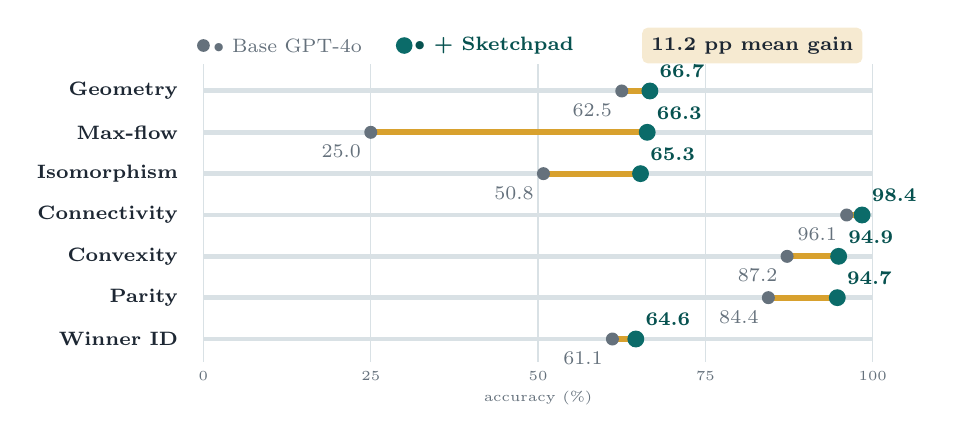
\begin{tikzpicture}[x=0.085cm,y=0.525cm]
      \foreach \x in {0,25,50,75,100}{
        \draw[MistDeep,line width=0.45pt] (\x,0.45) -- (\x,7.65);
        \node[font=\tiny,text=Muted] at (\x,0.10) {\x};
      }
      \node[anchor=west,font=\scriptsize,text=Muted] at (0,8.10) {$\bullet$ Base GPT-4o};
      \fill[Muted] (0,8.10) circle (2.3pt);
      \fill[Teal] (30,8.10) circle (3pt);
      \node[anchor=west,font=\scriptsize\bfseries,text=TealDark] at (30,8.10) {$\bullet$ + Sketchpad};
      \node[rounded corners=2pt,fill=Saffron!22,font=\scriptsize\bfseries,text=Ink]
        at (82,8.10) {11.2 pp mean gain};

      \resultrow{Geometry}{62.5}{66.7}{7}
      \resultrow{Max-flow}{25.0}{66.3}{6}
      \resultrow{Isomorphism}{50.8}{65.3}{5}
      \resultrow{Connectivity}{96.1}{98.4}{4}
      \resultrow{Convexity}{87.2}{94.9}{3}
      \resultrow{Parity}{84.4}{94.7}{2}
      \resultrow{Winner ID}{61.1}{64.6}{1}
      \node[font=\tiny,text=Muted] at (50,-0.42) {accuracy (\%)};
    \end{tikzpicture}
  \end{center}
\end{frame}

% 14 — VISION RESULTS
\begin{frame}{Sketchpad improves GPT-4o on every tested task}
  \vspace{-0.03cm}
  \begin{center}
    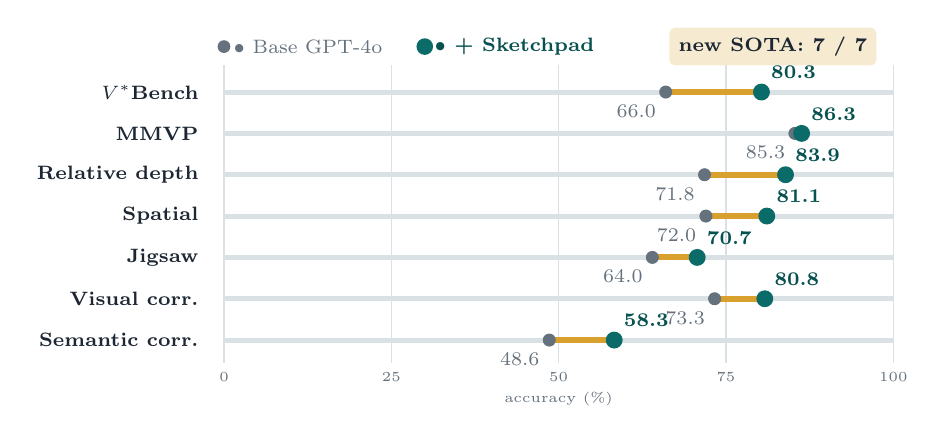
\begin{tikzpicture}[x=0.085cm,y=0.525cm]
      \foreach \x in {0,25,50,75,100}{
        \draw[MistDeep,line width=0.45pt] (\x,0.45) -- (\x,7.65);
        \node[font=\tiny,text=Muted] at (\x,0.10) {\x};
      }
      \fill[Muted] (0,8.10) circle (2.3pt);
      \node[anchor=west,font=\scriptsize,text=Muted] at (0,8.10) {$\bullet$ Base GPT-4o};
      \fill[Teal] (30,8.10) circle (3pt);
      \node[anchor=west,font=\scriptsize\bfseries,text=TealDark] at (30,8.10) {$\bullet$ + Sketchpad};
      \node[rounded corners=2pt,fill=Saffron!22,font=\scriptsize\bfseries,text=Ink]
        at (82,8.10) {new SOTA: 7 / 7};

      \resultrow{$V^*$Bench}{66.0}{80.3}{7}
      \resultrow{MMVP}{85.3}{86.3}{6}
      \resultrow{Relative depth}{71.8}{83.9}{5}
      \resultrow{Spatial}{72.0}{81.1}{4}
      \resultrow{Jigsaw}{64.0}{70.7}{3}
      \resultrow{Visual corr.}{73.3}{80.8}{2}
      \resultrow{Semantic corr.}{48.6}{58.3}{1}
      \node[font=\tiny,text=Muted] at (50,-0.42) {accuracy (\%)};
    \end{tikzpicture}
  \end{center}
\end{frame}

% 15 — EXAMPLES
\begin{frame}{Different visual primitives for different failures}
  \centering
  \vspace{0.04cm}
  \includegraphics[height=0.615\textheight]{examples.pdf}
\end{frame}

% 16 — COMPARISON
\begin{frame}{The only augmentation that improves every task}
  \vspace{0.18cm}
  \begin{center}
    {\small Change from the same GPT-4o baseline, in accuracy points}\par
    \vspace{0.22cm}
    \renewcommand{\arraystretch}{1.32}
    \setlength{\tabcolsep}{0.44cm}
    \begin{tabular}{lcccc}
      \toprule
      \textbf{Augmentation} & \textbf{$V^*$Bench} & \textbf{MMVP} & \textbf{Depth} & \textbf{Spatial} \\
      \midrule
      SoM & \downcell{-17.0} & \downcell{-14.6} & \downcell{-8.9} & \upcell{11.2} \\
      SoM + original & \upcell{2.1} & \downcell{-1.3} & \upcell{3.2} & \upcell{10.5} \\
      Visprog & \downcell{-33.6} & \downcell{-68.0} & \downcell{-25.0} & \downcell{-34.2} \\
      \rowcolor{Saffron!15}
      \textbf{Visual Sketchpad} & \textbf{\textcolor{TealDark}{+14.3}} &
        \textbf{\textcolor{TealDark}{+1.0}} & \textbf{\textcolor{TealDark}{+12.1}} &
        \textbf{\textcolor{TealDark}{+9.1}} \\
      \bottomrule
    \end{tabular}
  \end{center}
  \vspace{0.10cm}
  \begin{center}
    \goldpill{Fixed prompts can confuse}\hspace{0.20cm}
    \goldpill{Fixed programs propagate errors}\hspace{0.20cm}
    \pill{Sketchpad inspects and replans}
  \end{center}
\end{frame}

% 17 — ANALYSIS / HUMAN STUDY
\begin{frame}{The plans are sound; perception is the bottleneck}
  \begin{columns}[T,onlytextwidth]
    \column{0.52\textwidth}
      \eyebrow{Why it works}\par
      \vspace{0.24cm}
      \begin{enumerate}
        \setlength{\itemsep}{0.45cm}
        \item \textbf{Vision complements language.} Depth and masks preserve dense information.
        \item \textbf{Artifacts are inspectable.} The agent can react to a failed detection or an unhelpful sketch.
        \item \textbf{Plans resemble human strategies.} The model exploits familiar reasoning patterns.
      \end{enumerate}

    \column{0.44\textwidth}
      \begin{beamercolorbox}[rounded=true,wd=\linewidth,ht=2.08cm,dp=0.12cm,sep=0.28cm]{accent card}
        {\fontsize{27}{29}\selectfont\bfseries\textcolor{Saffron!85!black}{80\%}}\par
        {\small Humans draw the same auxiliary line as GPT-4o on geometry.}
      \end{beamercolorbox}
      \vspace{0.25cm}
      \begin{beamercolorbox}[rounded=true,wd=\linewidth,ht=2.08cm,dp=0.12cm,sep=0.28cm]{positive card}
        {\fontsize{27}{29}\selectfont\bfseries\textcolor{TealDark}{92.8\%}}\par
        {\small Human raters judge GPT-4o's full vision plan valid.}
      \end{beamercolorbox}
  \end{columns}
\end{frame}

% =============================================================================
\section{Implications}
% =============================================================================

% 18 — LIMITATIONS
\begin{frame}{Visual reasoning is capable, but not yet cheap}
  \vspace{0.18cm}
  \begin{columns}[T,onlytextwidth]
    \column{0.315\textwidth}
      \begin{beamercolorbox}[rounded=true,wd=\linewidth,ht=3.45cm,dp=0.12cm,sep=0.30cm]{negative card}
        \eyebrow{01 \; Cost}\par\vspace{0.20cm}
        {\bfseries More inference compute}\par\vspace{0.20cm}
        {\small Code execution and specialist calls cost more than directly emitting language tokens.}
      \end{beamercolorbox}
    \column{0.315\textwidth}
      \begin{beamercolorbox}[rounded=true,wd=\linewidth,ht=3.45cm,dp=0.12cm,sep=0.30cm]{negative card}
        \eyebrow{02 \; Reliability}\par\vspace{0.20cm}
        {\bfseries Tool errors remain}\par\vspace{0.20cm}
        {\small Detection, segmentation, and simple visual QA can still fail. Replanning helps, but does not eliminate them.}
      \end{beamercolorbox}
    \column{0.315\textwidth}
      \begin{beamercolorbox}[rounded=true,wd=\linewidth,ht=3.45cm,dp=0.12cm,sep=0.30cm]{accent card}
        \eyebrow{03 \; Opportunity}\par\vspace{0.20cm}
        {\bfseries Train models to sketch natively}\par\vspace{0.20cm}
        {\small Future multimodal models could learn when and how to generate visual intermediate states.}
      \end{beamercolorbox}
  \end{columns}
  \vspace{0.42cm}
  \begin{center}\pill{robotic search}\hspace{0.22cm}\pill{navigation}\hspace{0.22cm}\pill{manipulation}\end{center}
\end{frame}

% 19 — TAKEAWAYS
\begin{frame}{A useful chain of thought need not be a chain of words}
  \vspace{0.14cm}
  \begin{center}
    {\fontsize{12}{16}\selectfont\bfseries
     Visual Sketchpad makes \textcolor{Teal}{drawing} an explicit,
     inspectable part of multimodal reasoning.}
  \end{center}
  \vspace{0.26cm}
  \begin{columns}[T,onlytextwidth]
    \column{0.315\textwidth}
      \begin{beamercolorbox}[rounded=true,wd=\linewidth,ht=2.35cm,dp=0.15cm,sep=0.27cm]{card}
        \eyebrow{Mechanism}\par\vspace{0.14cm}
        \textbf{Plan $\rightarrow$ draw $\rightarrow$ inspect $\rightarrow$ adapt}
      \end{beamercolorbox}
    \column{0.315\textwidth}
      \begin{beamercolorbox}[rounded=true,wd=\linewidth,ht=2.35cm,dp=0.15cm,sep=0.27cm]{positive card}
        \eyebrow{Result}\par\vspace{0.14cm}
        \textbf{Consistent gains across math and all seven visual tasks}
      \end{beamercolorbox}
    \column{0.315\textwidth}
      \begin{beamercolorbox}[rounded=true,wd=\linewidth,ht=2.35cm,dp=0.15cm,sep=0.27cm]{accent card}
        \eyebrow{Implication}\par\vspace{0.14cm}
        \textbf{Intermediate representations should match the structure of the problem}
      \end{beamercolorbox}
  \end{columns}
  \vspace{0.55cm}
  \begin{center}
    {\small\bfseries Thank you}\qquad
    \href{https://visualsketchpad.github.io/}{\textcolor{Teal}{visualsketchpad.github.io}}
  \end{center}
\end{frame}

% 20 — REFERENCES
\section{References}
\begin{frame}{Selected references}
  \setbeamertemplate{bibliography item}[text]
  \scriptsize
  \setlength{\parskip}{0.16cm}
  \begin{thebibliography}{99}
    \bibitem{hu2024} Hu, Y., Shi, W., Fu, X., et al. (2024).
      Visual Sketchpad: Sketching as a Visual Chain of Thought for Multimodal Language Models.
      \emph{NeurIPS 2024}.
    \bibitem{wei2022} Wei, J., et al. (2022).
      Chain-of-Thought Prompting Elicits Reasoning in Large Language Models. \emph{NeurIPS}.
    \bibitem{yao2023} Yao, S., et al. (2023).
      ReAct: Synergizing Reasoning and Acting in Language Models. \emph{ICLR}.
    \bibitem{fu2024iso} Fu, X., et al. (2024).
      IsoBench: Benchmarking Multimodal Foundation Models on Isomorphic Representations. \emph{COLM}.
    \bibitem{fu2024blink} Fu, X., et al. (2024).
      BLINK: Multimodal Large Language Models Can See but Not Perceive. \emph{ECCV}.
    \bibitem{wu2024vstar} Wu, P. and Xie, S. (2024).
      $V^*$: Guided Visual Search as a Core Mechanism in Multimodal LLMs. \emph{CVPR}.
    \bibitem{yang2023som} Yang, J., et al. (2023).
      Set-of-Mark Prompting Unleashes Visual Grounding in GPT-4V. \emph{arXiv}.
    \bibitem{gupta2023} Gupta, T. and Kembhavi, A. (2023).
      Visual Programming: Compositional Visual Reasoning without Training. \emph{CVPR}.
    \bibitem{wu2023autogen} Wu, Q., et al. (2023).
      AutoGen: Enabling Next-Gen LLM Applications via Multi-Agent Conversation. \emph{arXiv}.
  \end{thebibliography}
  \vfill
  {\color{Muted}\fontsize{6.8}{8}\selectfont
   Paper, code, and project assets: \url{https://visualsketchpad.github.io/}}
\end{frame}

\end{document}
